\subsubsection{10.02.2016}
\textit{\textbf{Time frame:}} 19:00-21:00 

Today it was installed the second section of the mechanism for pushing the “All Clear” signal. Then the mechanism was tested (figure \ref{PushSig1.3}, \ref{PushSig1.4}). The result of the test was positive.

\begin{figure}[H]
	\begin{minipage}[h]{0.47\linewidth}
		\center{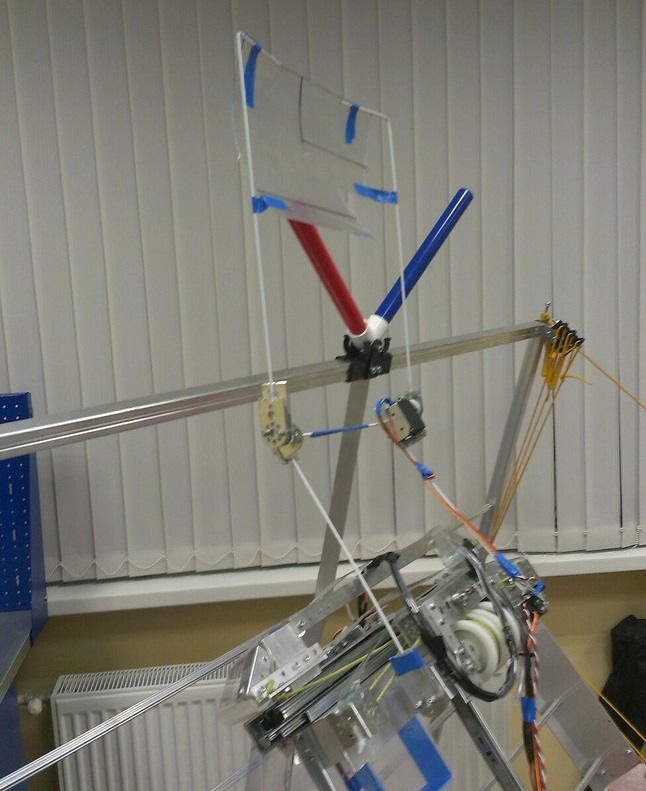
\includegraphics[scale=0.2]{3Engineering/5Team_meetings/days_of_meetings/2016.02.10/images/01}}
		\caption{How the mechanism works 1}
		\label{PushSig1.3}
	\end{minipage}
	\hfill
	\begin{minipage}[h]{0.47\linewidth}
		\center{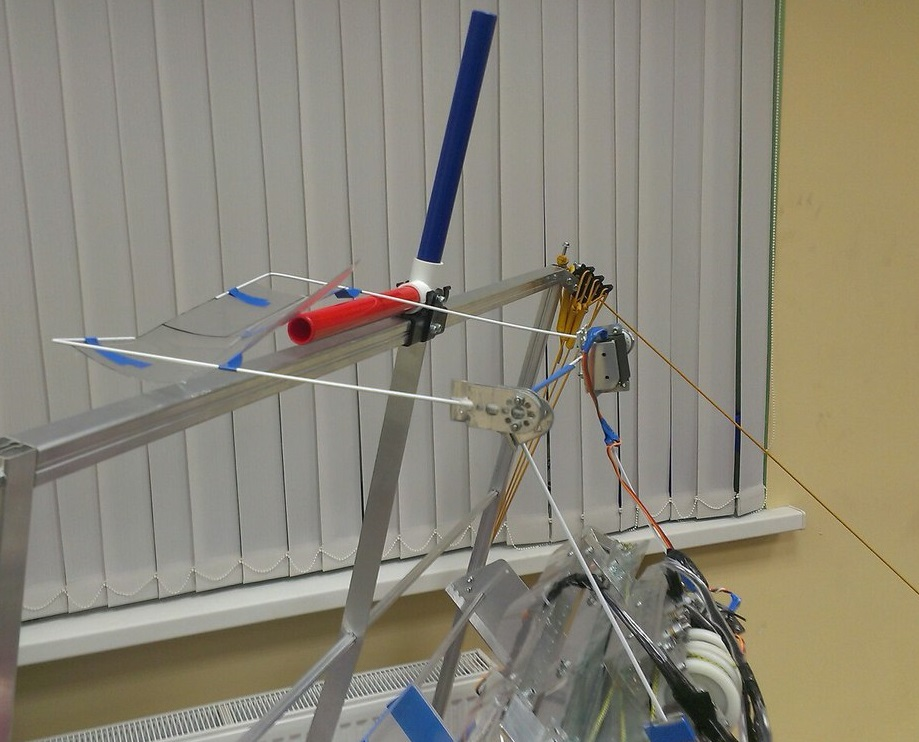
\includegraphics[scale=0.2]{3Engineering/5Team_meetings/days_of_meetings/2016.02.10/images/02}}
		\caption{How the mechanism works 2}
		\label{PushSig1.4}
	\end{minipage}
\end{figure}
